%%%%%%%%%%%%%%%%%%%%%%%%%%%%%%%%%%%%%%%%%%%%%%%%%%%%%%%
%%      Para começar a usar este template, primeiro, %%
%% você dever criar uma conta no ShareLates. Depois, %%
%% vá nasopções no canto esquerdo superior da tela e %%
%% clique em "Copiar Projeto". Dê um novo nome para  %%
%% o projeto. This work has the LPPL maintenance     %%
%% status `maintained' The Currentt Maintainer of    %%
%% this work are:                                    %%
%%                                                   %%
%%        Ednardo Moreira Rodrigues (UFC/DEE)        %%
%%                      and                          %%
%%        Alan Batista de Oliveira (UFC/DEE)         %%
%%                                                   %%
%% Review:                                           %%
%%                                                   %%
%% - Eliene Maria Vieira de Moura;                   %%
%% - Francisco Edvander Pires Santos;                %%  
%% - Izabel Lima dos Santos;                         %%
%% - Juliana Soares Lima;                            %%
%% - Kalline Yasmin Soares Feitosa.                  %%
%%                                                   %%
%% This work may be distributed and/or modified under%%
%% theconditions of the LaTeX Project Public License,%%
%% either version 1.3 of this license or (at your    %%
%% option) any                                       %%
%% later version. The latest version of this license %%
%% is in http://www.latex-project.org/lppl.txt and   %%
%% version 1.3 or later is part of all distributions %%
%% of LaTeX version 2005/12/01 or later.             %%
%% The First Maintainer of this work was:            %%
%% Thiago Nascimento  (UECE)                         %%
%% Project available on:                             %%
%% https://github.com/thiagodnf/uecetex2             %%
%% Further information about abnTeX2                 %%
%% are available on http://abntex2.googlecode.com/   %%
%%%%%%%%%%%%%%%%%%%%%%%%%%%%%%%%%%%%%%%%%%%%%%%%%%%%%%%

\documentclass[        
    a4paper,          % Tamanho da folha A4
    12pt,             % Tamanho da fonte 12pt
    chapter=TITLE,    % Todos os capitulos devem ter caixa alta
    section=Title,    % Todas as secoes devem ter caixa alta somente na primeira letra
    subsection=Title, % Todas as subsecoes devem ter caixa alta somente na primeira letra
    oneside,          % Usada para impressao em apenas uma face do papel
    english,          % Hifenizacoes em ingles
    spanish,          % Hifenizacoes em espanhol
    brazil,           % Ultimo idioma eh o idioma padrao do documento
    fleqn             % Coloca as equações alinhadas a esquerda
]{abntex2}

%%%%%%%%%%%%%%%%%%%%%%%%%%%%%%%%%%%%%%%%%%%%%%%%%%%%%%%
%%      Para começar a usar este template, primeiro, %%
%% você dever criar uma conta no ShareLates. Depois, %%
%% vá nasopções no canto esquerdo superior da tela e %%
%% clique em "Copiar Projeto". Dê um novo nome para  %%
%% o projeto. This work has the LPPL maintenance     %%
%% status `maintained' The Currentt Maintainer of    %%
%% this work are:                                    %%
%%                                                   %%
%%        Ednardo Moreira Rodrigues (UFC/DEE)        %%
%%                      and                          %%
%%        Alan Batista de Oliveira (UFC/DEE)         %%
%%                                                   %%
%% Review:                                           %%
%%                                                   %%
%% - Eliene Maria Vieira de Moura;                   %%
%% - Francisco Edvander Pires Santos;                %%  
%% - Izabel Lima dos Santos;                         %%
%% - Juliana Soares Lima;                            %%
%% - Kalline Yasmin Soares Feitosa.                  %%
%%                                                   %%
%% This work may be distributed and/or modified under%%
%% theconditions of the LaTeX Project Public License,%%
%% either version 1.3 of this license or (at your    %%
%% option) any                                       %%
%% later version. The latest version of this license %%
%% is in http://www.latex-project.org/lppl.txt and   %%
%% version 1.3 or later is part of all distributions %%
%% of LaTeX version 2005/12/01 or later.             %%
%% The First Maintainer of this work was:            %%
%% Thiago Nascimento  (UECE)                         %%
%% Project available on:                             %%
%% https://github.com/thiagodnf/uecetex2             %%
%% Further information about abnTeX2                 %%
%% are available on http://abntex2.googlecode.com/   %%
%%%%%%%%%%%%%%%%%%%%%%%%%%%%%%%%%%%%%%%%%%%%%%%%%%%%%%%

% \documentclass[        
%     a4paper,          % Tamanho da folha A4
%     12pt,             % Tamanho da fonte 12pt
%     chapter=TITLE,    % Todos os capitulos devem ter caixa alta
%     section=TITLE,    % Todas as secoes devem ter caixa alta
%     oneside,          % Usada para impressao em apenas uma face do papel
%     english,          % Hifenizacoes em ingles
%     spanish,          % Hifenizacoes em espanhol
%     brazil            % Ultimo idioma eh o idioma padrao do documento
% ]{abntex2}

% Importações de pacotes
% possibilita ctrl+c com acentos em português
\usepackage[utf8]{inputenc}                         % Acentuação direta
\usepackage[T1]{fontenc}                            % Codificação da fonte em 8 bits
\usepackage{graphicx}                               % Inserir figuras
\usepackage{amsfonts, amssymb, amsmath}             % Fonte e símbolos matemáticos
\usepackage{booktabs}                               % Comandos para tabelas
\usepackage{verbatim}                               % Texto é interpretado como escrito no documento
\usepackage{multirow, array}                        % Múltiplas linhas e colunas em tabelas
\usepackage{indentfirst}                            % Endenta o primeiro parágrafo de cada seção.
\usepackage{listings}                               % Utilizar codigo fonte no documento
\usepackage{xcolor}
\usepackage{microtype}                              % Para melhorias de justificação?
\usepackage[portuguese,ruled,lined]{algorithm2e}    % Escrever algoritmos
\usepackage{algorithmic}                            % Criar Algoritmos  
%\usepackage{float}                                 % Utilizado para criação de floats
\usepackage{amsgen}
\usepackage{lipsum}                                 % Usar a simulação de texto Lorem Ipsum
%\usepackage{titlesec}                              % Permite alterar os títulos do documento
\usepackage{tocloft}                                % Permite alterar a formatação do Sumário
\usepackage{etoolbox}                               % Usado para alterar a fonte da Section no Sumário
\usepackage[acronym,nogroupskip,nonumberlist]{glossaries}   % Permite fazer o glossario
\usepackage[font=singlespacing]{caption}                                % Altera o comportamento da tag caption
\usepackage[alf, abnt-emphasize=bf, recuo=0cm, abnt-etal-cite=2, abnt-etal-list=0, abnt-etal-text=it]{abntex2cite}  % Citações padrão ABNT
%\usepackage[bottom]{footmisc}                      % Mantém as notas de rodapé sempre na mesma posição
%\usepackage{times}                                 % Usa a fonte Times
\usepackage{mathptmx}                               % Usa a fonte Times New Roman										
%\usepackage{lmodern}                               % Usa a fonte Latin Modern
%\usepackage{subfig}                                % Posicionamento de figuras
%\usepackage{scalefnt}                              % Permite redimensionar tamanho da fonte
%\usepackage{color, colortbl}                       % Comandos de cores
%\usepackage{lscape}                                % Permite páginas em modo "paisagem"
\usepackage{ae, aecompl}                            % Fontes de alta qualidade
%\usepackage{picinpar}                              % Dispor imagens em parágrafos
\usepackage{latexsym}                               % Símbolos matemáticos
%\usepackage{upgreek}                               % Fonte letras gregas
\usepackage{appendix}                               % Gerar o apendice no final do documento
\usepackage{paracol}                                % Criar paragrafos sem identacao
\usepackage{lib/ufctex}		                        % Biblioteca com as normas da UFC para trabalhos academicos
\usepackage{pdfpages}                               % Incluir pdf no documento
\usepackage{amsmath}                                % Usar equacoes matematicas


% Meus Pacotes - Não pertencem ao template original
% adicionar os simbolos dos question\'arios
\usepackage{threeparttable}
\usepackage{wasysym}
\usepackage{float}

% Organiza e gera a lista de abreviaturas, simbolos e glossario
\makeglossaries

% Gera o Indice do documento
\makeindex


%%%%%%%%%%%%%%%%%%%%%%%%%%%%%%%%%%%%%%%%%%%%%%%%%%%%%
%%          Configuracoes do ufctex                %%
%%%%%%%%%%%%%%%%%%%%%%%%%%%%%%%%%%%%%%%%%%%%%%%%%%%%%

% Opcoes disponiveis

\trabalhoacademico{tccgraduacao}
%\trabalhoacademico{tccespecializacao}
%\trabalhoacademico{dissertacao}
%\trabalhoacademico{tese}

% Define se o trabalho eh uma qualificacao
% Coloque 'nao' para versao final do trabalho

\ehqualificacao{nao}

% Remove as bordas vermelhas e verdes do PDF gerado
% Coloque 'sim' pare remover

\removerbordasdohyperlink{sim} 

% Adiciona a cor Azul a todos os hyperlinks

\cordohyperlink{nao}

%%%%%%%%%%%%%%%%%%%%%%%%%%%%%%%%%%%%%%%%%%%%%%%%%%%%%
%%          Informação sobre a IES                 %%
%%%%%%%%%%%%%%%%%%%%%%%%%%%%%%%%%%%%%%%%%%%%%%%%%%%%%

\ies{Universidade Federal do Ceará}
\iessigla{UFC}
\centro{Centro de Xxxxxxxx}

%%%%%%%%%%%%%%%%%%%%%%%%%%%%%%%%%%%%%%%%%%%%%%%%%%%%%
%%        Informação para TCC de Graduacao %%
%%%%%%%%%%%%%%%%%%%%%%%%%%%%%%%%%%%%%%%%%%%%%%%%%%%%%

\graduacaoem{Engenharia Xxxxxxx}
\habilitacao{bacharel} % Pode colocar tambem 'licenciada'

%%%%%%%%%%%%%%%%%%%%%%%%%%%%%%%%%%%%%%%%%%%%%%%%%%%%%
%%     Informação para TCC de Especializacao       %%
%%%%%%%%%%%%%%%%%%%%%%%%%%%%%%%%%%%%%%%%%%%%%%%%%%%%%

\especializacaoem{Descargas Atmosféricas}

%%%%%%%%%%%%%%%%%%%%%%%%%%%%%%%%%%%%%%%%%%%%%%%%%%%%%
%%         Informação para Dissertacao             %%
%%%%%%%%%%%%%%%%%%%%%%%%%%%%%%%%%%%%%%%%%%%%%%%%%%%%%

\programamestrado{Programa de Pós-Graduação em Xxxxxxx}
\nomedomestrado{Mestrado Acadêmico em Xxxxxxx}
\mestreem{Engenharia Xxxxxx}
\areadeconcentracaomestrado{Engenharia Xxxxxx}

%%%%%%%%%%%%%%%%%%%%%%%%%%%%%%%%%%%%%%%%%%%%%%%%%%%%%
%%               Informação para Tese              %%
%%%%%%%%%%%%%%%%%%%%%%%%%%%%%%%%%%%%%%%%%%%%%%%%%%%%%

\programadoutorado{Programa de Pós-Graduação em Xxxxxx}
\nomedodoutorado{Doutorado em Xxxxxxx}
\doutorem{Engenharia Xxxxxx}
\areadeconcentracaodoutorado{Engenharia Xxxxxxx}

%%%%%%%%%%%%%%%%%%%%%%%%%%%%%%%%%%%%%%%%%%%%%%
%%  Informacoes relacionadas ao trabalho     %%
%%%%%%%%%%%%%%%%%%%%%%%%%%%%%%%%%%%%%%%%%%%%%%

\autor{Nome Sobrenome}
\titulo{Título do Trabalho}
\data{2016}
\local{Fortaleza}

% Exemplo: \dataaprovacao{01 de Janeiro de 2012}
\dataaprovacao{}

%%%%%%%%%%%%%%%%%%%%%%%%%%%%%%%%%%%%%%%%%%%%%
%%     Informação sobre o Orientador       %%
%%%%%%%%%%%%%%%%%%%%%%%%%%%%%%%%%%%%%%%%%%%%%

\orientador{Prof. Dr. Xxxxxxx Xxxxxx Xxxxxxx}
\orientadories{Universidade Federal do Ceará (UFC)}
\orientadorcentro{Centro de Ciências e Tecnologia (CCT)}
\orientadorfeminino{nao} % Coloque 'sim' se for do sexo feminino

%%%%%%%%%%%%%%%%%%%%%%%%%%%%%%%%%%%%%%%%%%%%%
%%      Informação sobre o Co-orientador   %%
%%%%%%%%%%%%%%%%%%%%%%%%%%%%%%%%%%%%%%%%%%%%%

% Deixe o nome do coorientador em branco para remover do documento

\coorientador{}
\coorientadories{Universidade Co-orientador (SIGLA)}
\coorientadorcentro{Centro do Co-orientador (SIGLA)}
\coorientadorfeminino{nao} % Coloque 'sim' se for do sexo feminino

%%%%%%%%%%%%%%%%%%%%%%%%%%%%%%%%%%%%%%%%%%%%%
%%      Informação sobre a banca           %%
%%%%%%%%%%%%%%%%%%%%%%%%%%%%%%%%%%%%%%%%%%%%%

% Atenção! Deixe o nome do membro da banca para remover da folha de aprovacao

% Exemplo de uso:
% \membrodabancadois{Prof. Dr. Fulano de Tal}
% \membrodabancadoisies{Universidade Federal do Ceará - UFC}

\membrodabancadois{Prof. Dr. Xxxxxxx Xxxxxx Xxxxxxx}
\membrodabancadoiscentro{Faculdade de Filosofia Dom Aureliano Matos (FAFIDAM)}
\membrodabancadoisies{Universidade do Membro da Banca Dois (SIGLA)}
\membrodabancatres{Prof. Dr. Xxxxxxx Xxxxxx Xxxxxxx}
\membrodabancatrescentro{Centro de Ciências e Tecnologia (CCT)}
\membrodabancatresies{Universidade do Membro da Banca Três (SIGLA)}
\membrodabancaquatro{Prof. Dr. Xxxxxxx Xxxxxx Xxxxxxx}
\membrodabancaquatrocentro{Centro de Ciências e Tecnologia (CCT)}
\membrodabancaquatroies{Universidade do Membro da Banca Quatro (SIGLA)}
\membrodabancacinco{Prof. Dr. Xxxxxxx Xxxxxx Xxxxxxx}
\membrodabancacincocentro{Teste}
\membrodabancacincoies{Universidade do Membro da Banca Cinco (SIGLA)}
\membrodabancaseis{Prof. Dr. Xxxxxxx Xxxxxx Xxxxxxx}
\membrodabancaseiscentro{}
\membrodabancaseisies{Universidade do Membro da Banca Seis (SIGLA)}

\begin{document}	

	% Elementos pré-textuais
	\imprimircapa
	\imprimirfolhaderosto{}
	\imprimirfichacatalografica{elementos-pre-textuais/ficha-catalografica}
	%\imprimirerrata{elementos-pre-textuais/errata}
	\imprimirfolhadeaprovacao
	\imprimirdedicatoria{elementos-pre-textuais/dedicatoria}
	\imprimiragradecimentos{elementos-pre-textuais/agradecimentos}
	\imprimirepigrafe{elementos-pre-textuais/epigrafe}
	\imprimirresumo{elementos-pre-textuais/resumo}
	\imprimirabstract{elementos-pre-textuais/abstract}
	\imprimirlistadeilustracoes
	\imprimirlistadetabelas
	%\imprimirlistadequadros
	%\imprimirlistadealgoritmos
	%\imprimirlistadecodigosfonte
	\imprimirlistadeabreviaturasesiglas
	\imprimirlistadesimbolos{elementos-pre-textuais/lista-de-simbolos}   
	\imprimirsumario
	
	%Elementos textuais
	\textual
	\chapter{INTRODUÇÃO}
\label{cap:introducao}

A Matemática, como ciência, tem uma relação muito especial com as novas tecnologias desde as calculadoras aos computadores, sistemas 
multim\'idia, e a \textit{Internet}. No entanto, alguns professores costumam demorar a perceber como tirar proveito destas tecnologias como 
ferramentas de trabalho \cite{da1997ensino}. \`A medida que a quantidade de recursos tecnológicos na sala de aula foram aumentando, 
tornou-se conveniente a criação de novas metodologias de ensino, especificamente na Educação Matemática. A busca por novas 
metodologias de ensino que fazem uso destes recursos procura fazer da matemática uma disciplina atraente e desvinculada do ensino 
tradicional, que já se mostrou ineficiente \cite{silva2009ambiente}.

Grande parte dos alunos, em todas as faixas etárias, tem dificuldades em aprender matemática, e muitas vezes essas dificuldades ocorrem 
não pela falta de atenção ou por não gostar do conteúdo, mas por fatores mentais, psicológicos e pedag\'ogicos que envolvem uma série de 
trabalhos e conceitos que 
precisam ser desenvolvidos \cite{de2006dificuldades}. Mas como auxiliar alunos com dificuldades na aprendizagem da matemática? Em busca 
dessa resposta, diferentes sistemas de \textit{software} foram desenvolvidos buscando servir \`a  educação Matem\'atica. Em 2006, Salman 
Khan fundou a Khan Academy, uma organização educacional que tem por objetivo oferecer exercícios, vídeos de instrução e um painel de 
aprendizado personalizado que habilita os estudantes a aprender no seu próprio ritmo dentro e fora da sala de aula \cite{khan2012one}. A 
plataforma criada por Khan utiliza vídeo-aulas e resolução de problemas para ensinar seus alunos, permitindo que cada um aprenda de forma 
independente e no seu pr\'oprio ritmo. Uma outra plataforma também  importante nessa área, \'e o ActiveMath 
\cite{melis2001activemath}, uma plataforma que permite aos estudantes desfrutarem da experiência de estudar num 
curso gerado dinamicamente. Nessa plataforma, os conte\'udos s\~ao representados no formato XML \cite{bray1998extensible} e armazenados 
numa base de conhecimento\footnote{São bases de dados ou conhecimentos acumulados sobre um determinado assunto.}, onde s\~ao recuperados para gerar cursos individuais de acordo com regras 
pedagógicas\footnote{S\~ao regras que determinam quando e quais ferramentas do sistema devem ser apresentadas e em que ordem.} 
\cite{melis2004activemath}. Estes e outros trabalhos serão apresentados com mais detalhes na \autoref{cap:trabalhos-relacionados}.

O presente trabalho apresenta o projeto de um \gls{ava} \cite{valentini2010aprendizagem}, para auxiliar 
estudantes no ensino e aprendizagem de conteúdos matemáticos. Este ambiente se propõe a servir como ferramenta para estudantes que buscam 
estudar fora do ambiente escolar e em seu próprio ritmo. O ambiente também dará suporte ao ensino e aprendizagem em sala de aula, 
auxiliando professores com informações relevantes sobre o andamento do aprendizado de cada um de seus alunos, além das dificuldades que os 
mesmos apresentam.

A ideia deste AVA surgiu quando professores das disciplinas de matemática da Universidade Federal do Cear\'a observaram um grande número de 
reprovações e desistências em suas turmas. Segundo os professores, um dos fatores que pode ser o causador são as deficiências de formação em 
matemática desde o ensino médio, e, por isso, faltaria aos alunos a base para compreender os novos assuntos. Essa suspeita é reforçada por 
um estudo realizado pela Organização para a Cooperação e Desenvolvimento Econômico \cite{pisainfocus2016}. Esse estudo revelou que 67.1\% 
dos alunos brasileiros ainda estavam abaixo do nível 2 (os níveis são de 1 a 6) de proficiência em matem\'atica, deixando o país em 58º 
lugar 
na escala do PISA\footnote{O 
Programa Internacional de Avaliação de Estudantes (Pisa) é uma iniciativa de avaliação comparada, aplicada a estudantes na faixa dos 15 
anos, idade em que se pressupõe o término da escolaridade básica obrigatória na maioria dos países e que visa melhorar as políticas e 
resultados educacionais.}, ficando na frente apenas de países como Jordânia, Catar, Colômbia, Peru e Indonésia na \'ultima posi\c{c}\~ao. 
Sendo que somente 0,8\% dos estudantes brasileiros alcançaram os últimos patamares.

\section{Objetivos do Trabalho}

Este trabalho objetiva apresentar o projeto de um AVA para auxiliar no processo de ensino e aprendizagem de matemática por alunos dentro e 
fora da sala de aula, buscando contribuir com o processo de ensino e aprendizagem de matem\'atica. 

Como objetivos específicos para este trabalho, temos: 
[DEIXA PRA FAZER COM O SAMY]
\begin{alineas}
  \item Levantar os requisitos do sistema.
  \item Desenvolver os módulos com funções de administração do sistema.
  \item Desenvolver os módulos com funções que serão utilizadas pelos estudantes aplicando técnicas de Gamificação.
  \item Avaliar a interface do ambiente desenvolvido aplicando um teste de usabilidade com estudantes do ensino m\'edio e universit\'arios.
\end{alineas}


\section{Divisão do Trabalho}

Fundamentando-se na problemática mencionada e tendo em vista o objeto de estudo, dividimos esta monografia em quatro capítulos. No 
segundo cap\'itulo, destacaremos os aspectos teóricos sobre ensino e aprendizagem, assim como as tradicionais metodologias de ensino e as 
apoiadas por computador. Abordaremos tamb\'em conceitos de gamificação e os trabalhos que servem de refer\^encia para os conceitos e 
id\'eias utilizadas no trabalho aqui desenvolvido. No terceiro capítulo, discutiremos a concepção, construção e modelagem do sistema, 
apresentando o que o mesmo deve possuir e por que, e no quarto capítulo, apresentaremos os resultados alcan\c{c}ados.
	\chapter{Título do segundo capítulo}
\label{cap:fundamentacao-teorica}

    Alguns autores preferem fazer uma "fundamentação teórica" ~no segundo capítulo, outros, preferem fazer uma "revisão da literatura". Entretanto, isto é particular de cada trabalho e o autor deve escolher o título mais adequado. Consultar o orientador é importante para determinar o título apropriado.

    Evite começar da seção secundária, ou seja, não passe direto do título do capítulo para o título da seção secundária. Escreva um texto para introduzir as seções subsequentes. Lembre-se de utilizar primeira letra maiúscula quando estiver se referindo a um objeto com numeração específica como capítulo, seção, subseção, figura, tabela, quadro, equação, normalmente, se escreve a primeira letra maiúscula da palavra do objeto seguido do \textit{label}. Por exemplo, a Seção \ref{sec:citacoes} explica como fazer citações bibliográficas. Observe no código fonte deste texto como foi feita a referência cruzada. Isso permite enumerar a seção do modo automático o que facilita caso novas seções sejam criadas.  

    \section{Citações bibliográficas}
    \label{sec:citacoes}

        Esta frase mostra como citar um livro sobre descargas atmosféricas \cite{rakov2003lightning}. Também podem ser citados sites como \citeonline{elat2015densidade}.

        Referenciando outro site \cite{secretaria1999}. Texto texto texto texto texto texto texto texto texto texto texto texto texto texto texto texto texto texto texto. Texto texto texto texto texto texto texto texto texto texto texto texto texto texto texto texto texto texto texto. Texto texto texto texto texto texto texto texto texto texto texto texto texto texto texto texto texto texto texto. Texto texto texto texto texto texto texto texto texto texto texto texto texto texto texto texto texto texto texto. Citando uma norma \cite{NBR10520:1988}.
        
        Citação de duas referências que concordam entre si \cite{lamport1986latex,Maia2011}. Texto texto texto texto texto texto texto texto texto texto texto texto texto texto texto texto texto texto texto. Texto texto texto texto texto texto texto texto texto texto texto texto texto texto texto texto texto texto texto. Texto texto texto texto texto texto texto texto texto texto texto texto texto texto texto texto texto texto texto. Texto texto texto texto texto texto texto texto texto texto texto texto texto texto texto texto texto texto texto texto texto texto texto texto texto texto. Citando um manual \cite{manuais1989}. 
        
        Outro tipo de citação é a citação literal ou direta com mais de três linhas. Este tipo de citação deve ser destacada com recuo de $4~cm$ da margem esquerda com letra menor (tamanho 10), sem aspas e com espaçamento simples.  Para exemplificar esse tipo de citação, considere a afirmação de \citeonline{feitosa2016}:
        
        \begin{citacao}
            A cultura é o processo através do qual o homem cria o algo onde antes imperava o
            nada. Esse algo é toda complexidade de criações simbólicas, de sentidos e significados que
            damos às coisas e ao mundo. Um “algo” que não se sustenta se não se entender os processos
            culturais como mecanismos de mediação entre nós e os fenômenos. Assim, mais do que
            apenas um elemento da comunicação, a mediação é, por excelência, cultural. As diversas
            modalidades de mediação são apenas sotaques diferenciados dessa mediação cultural. Assim
            é a mediação informacional.
        \end{citacao}
        
        A afirmação do parágrafo anterior também pode ser reproduzida com a citação na final como mostra o exemplo a seguir: 
        
        \begin{citacao}
            A cultura é o processo através do qual o homem cria o algo onde antes imperava o
            nada. Esse algo é toda complexidade de criações simbólicas, de sentidos e significados que
            damos às coisas e ao mundo. Um “algo” que não se sustenta se não se entender os processos
            culturais como mecanismos de mediação entre nós e os fenômenos. Assim, mais do que
            apenas um elemento da comunicação, a mediação é, por excelência, cultural. As diversas
            modalidades de mediação são apenas sotaques diferenciados dessa mediação cultural. Assim
            é a mediação informacional \cite{feitosa2016}.
        \end{citacao}
        
        %Mais exemplos e opções de citações podem ser encontradas em:
        
%        https://en.wikibooks.org/wiki/LaTeX/Bibliography_Management
%        https://github.com/cfgnunes/latex-cefetmg/blob/master/latex-cefetmg/03-elementos-pos-textuais/apendices.tex        
        
        

    \section{Inserindo figuras}
    \label{sec:figuras}
    
    A Figura \ref{fig:reitoria} apresenta a fotografia da reitoria da Universidade Federal do Ceará. Observe a estrutura do código para inserir a Figura \ref{fig:reitoria}. No título, apenas a primeira letra da frase é maiúscula  exceto nomes próprios e não há ponto final. Procure ajustar o tamanho da figura para preencher a largura delimitada pelas margens esquerda e direita. Não esqueça de indicar fonte da figura. 
    
   	\begin{figure}[h!]
		\Caption{\label{fig:reitoria} Fotografia da Reitoria da Universidade Federal do Ceará}
		%\centering
		\UFCfig{}{
			\fbox{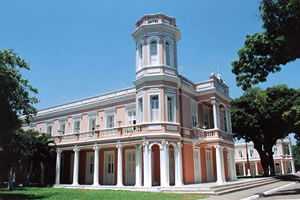
\includegraphics[width=12cm]{figuras/exemplo-1}}
		}{
			\Fonte{\citeonline{UFC2012}.}
		}	
	\end{figure}
	
    Texto texto texto texto texto texto texto texto texto texto texto texto texto texto texto texto texto texto texto texto texto texto texto texto texto texto texto texto texto texto texto texto texto texto texto texto texto texto texto texto texto texto texto texto texto.

    Texto texto texto texto texto texto texto texto texto texto texto texto texto texto texto texto texto texto texto. Texto texto texto texto texto texto texto texto texto texto texto texto texto texto texto texto texto texto texto.

    A Figura \ref{fig:sondas} Texto texto texto texto texto texto texto texto texto texto texto texto texto texto texto texto texto texto texto. Texto texto texto texto texto texto texto texto texto texto texto texto texto texto texto texto texto texto texto.

	\begin{figure}[h!]
		\centering
		\Caption{\label{fig:sondas} Gráfico da Atmosfera Superior}	
		\UFCfig{}{
			\fbox{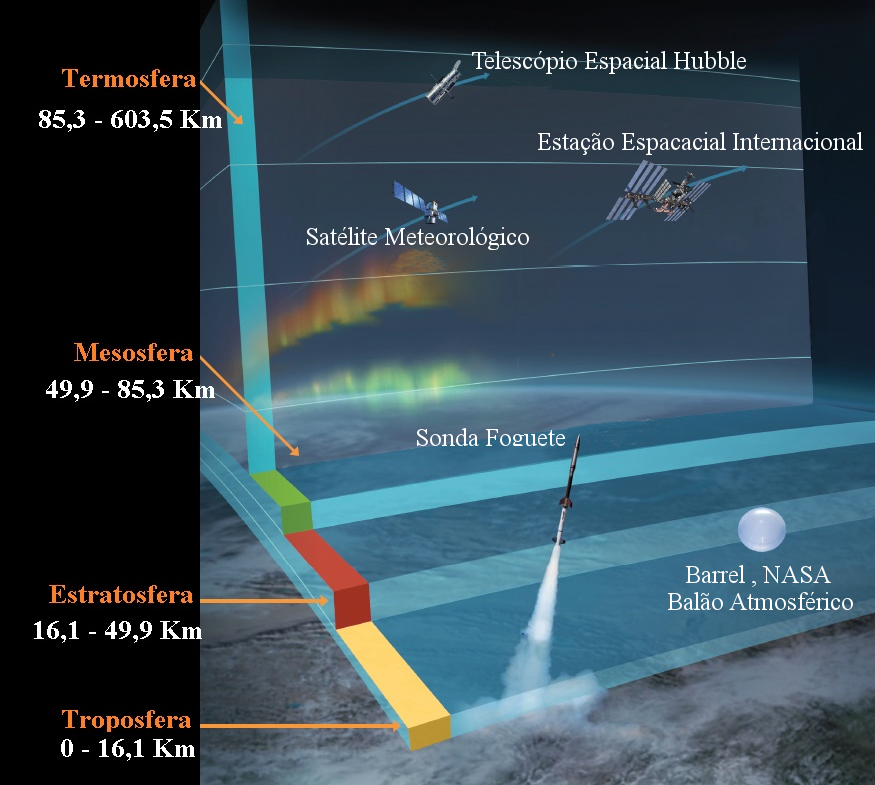
\includegraphics[width=12cm]{figuras/sondas}}
		}{
			\Fonte{adaptado de \citeonline{NASA2016}.}}	
	\end{figure}

    Texto texto texto texto texto texto texto texto texto texto texto texto texto texto texto texto texto texto texto texto texto texto texto texto texto texto texto texto texto texto texto texto texto texto texto texto texto texto texto texto texto texto texto texto texto.

    Texto texto texto texto texto texto texto texto texto texto texto texto texto texto texto texto texto texto texto texto texto texto texto texto texto texto texto texto texto texto texto texto texto texto texto texto texto texto texto texto texto texto texto texto texto.

    Texto texto texto texto texto texto texto texto texto texto texto texto texto texto texto texto texto texto texto texto texto texto texto texto texto texto texto texto texto texto texto texto texto texto texto texto texto texto texto texto texto texto texto texto texto.

    Texto texto texto texto texto texto texto texto texto texto texto texto texto texto texto texto texto texto texto texto texto texto texto texto texto texto texto texto texto texto texto texto texto texto texto texto texto texto texto texto texto texto texto texto texto.

    Texto texto texto texto texto texto texto texto texto texto texto texto texto texto texto texto texto texto texto texto texto texto texto texto texto texto texto texto texto texto texto texto texto texto texto texto texto texto texto texto texto texto texto texto texto.

    \section{Inserindo tabelas}
    \label{sec:tabelas}

	A Tabela \ref{tab:exemplo-1} Texto texto texto texto texto texto texto texto texto texto texto texto texto texto texto texto texto texto texto. Texto texto texto texto texto texto texto texto texto texto texto texto texto texto texto texto texto texto texto.
		
	\begin{table}[h!]	
		\centering
		\Caption{\label{tab:exemplo-1} Exemplo de tabela}	
		\UFCtab{}{
			\begin{tabular}{cll}
				\toprule
				Ranking & Exon Coverage & Splice Site Support \\
				\midrule \midrule
				E1 & Complete coverage by a single transcript & Both splice sites\\
				E2 & Complete coverage by more than a single transcript & Both splice sites\\
				E3 & Partial coverage & Both splice sites\\
				E4 & Partial coverage & One splice site\\
				E5 & Complete or partial coverage & No splice sites\\
				E6 & No coverage & No splice sites\\
				\bottomrule
			\end{tabular}
		}{
		\Fonte{elaborado pelo autor.}
	}
	\end{table}

\subsection{Exemplo de subseção} \label{sec:ex_sec}
	
Texto texto texto texto texto texto texto texto texto texto texto texto texto texto texto texto texto texto texto texto texto texto texto texto texto texto texto texto texto texto texto texto texto texto texto texto texto texto texto texto texto texto texto texto texto.

%acrlong{DATASUS},\acrlong{DNV},\acrlong{DO},\acrlong{ESF},\acrlong{IBGE},\acrlong{MFC},\acrlong{MI},\acrlong{MS},\acrlong{NV},\acrlong{ODM},\acrlong{OI},\acrlong{OMS},\acrlong{ONU},\acrlong{PNI},\acrlong{PSF},\acrlong{RIPSA},\acrlong{RN},\acrlong{SIM},\acrlong{SINASC},\acrlong{SUS},\acrlong{TMI},\acrlong{TMMFC}


\begin{alineascomponto}
	\item Integer non lacinia magna. Aenean tempor lorem tellus, non sodales nisl commodo ut
	\item Proin mattis placerat risus sit amet laoreet. Praesent sapien arcu, maximus ac fringilla efficitur, vulputate faucibus sem. Donec aliquet velit eros, sit amet elementum dolor pharetra eget
	\item Integer eget mattis libero. Praesent ex velit, pulvinar at massa vel, fermentum dictum mauris. Ut feugiat accumsan augue, et ultrices ipsum euismod vitae
	\begin{subalineascomponto}
		\item Integer non lacinia magna. Aenean tempor lorem tellus, non sodales nisl commodo ut
		\item Proin mattis placerat risus sit amet laoreet.
	\end{subalineascomponto}
\end{alineascomponto}

Teste de siglas \gls{TMMFC}, \gls{DA}, \gls{MCEG}
	\section{PROCEDIMENTOS METODOLÓGICOS}

Os procedimentos metodológicos definem as principais etapas realizadas para o desenvolvimento deste trabalho, incluindo as pesquisas, o desenvolvimento e avaliação do \textit{software}. Nas seções a 
seguir, descrevemos essas etapas.

\subsection{Definição do Processo}

Processos de \textit{software} são utilizados pelos engenheiros de \textit{software} para controlar e coordenar projetos de desenvolvimento de \textit{softwares} reais \cite{talma2006desenvolvimento}. 
\citeonline{padua2003engenharia} descreve um processo como um conjunto de passos parcialmente  ordenados, constituídos por atividades, métodos, práticas e transformações, usados para atingir uma meta. 
Desta forma, um modelo de processo de \textit{software} é uma descrição simplificada de um processo, sendo também uma representação abstrata do mesmo para explicar as diferentes abordagens de 
desenvolvimento \cite{sommerville2003engenharia}.

Processos de software são complexos e dependem do julgamento humano como em qualquer processo intelectual. Sendo assim, não existe um processo de software ideal, todos são desenvolvidos de maneiras 
diferentes por cada organização \cite{sommerville2003engenharia}.

O processo de \textit{software} utilizado para desenvolver o sistema foi baseado no modelo cascata, também chamado de ciclo de vida clássico, proposto por Royce em 1970. Neste modelo, as fases são 
sistematicamente seguidas de maneira sequencial \cite{pressman2006engenharia}. O modelo inicia com a fase de especificação de requisitos, passando pelo planejamento, modelagem, construção e 
implantação, finalizando na manutenção progressiva do software, como apresentamos no \nameref{figura_ciclo_cascata}.

As vantagens desse modelo se devem ao fato de que só se avança para a tarefa seguinte quando o cliente valida e aceita os produtos finais da tarefa atual, facilitando assim a compreensão adquirida ao 
longo do projeto, além de facilitar o processo de criação da documentação para o sistema \cite{pressman2006engenharia}. Já as principais desvantagens, segundo \citeonline{pressman2006engenharia}, se 
devem ao fato de que os projetos reais raramente seguem o fluxo sequencial ao qual o modelo propõe. Este modelo exige ainda que todos os requisitos sejam estabelecidos na fase 
inicial, fato que geralmente é difícil tanto para o cliente quanto para o desenvolvedor, pois os requisitos geralmente est\~ao em constante mudan\c{c}a. Outro grande problema com esse modelo é que o 
cliente só recebe uma versão executável do sistema no final de todo o processo de desenvolvimento, o que não agrada a muitos clientes.

Levando em consideração as vantagens e desvantagens antes citadas, esse modelo foi escolhido como base para o processo por facilitar o desenvolvimento de uma documentação mais detalhada e 
principalmente pela equipe de desenvolvimento ser formada por uma única pessoa, o autor deste trabalho, impossibilitando a divisão de tarefas característica de metodologias 
ágeis \footnote{Metodologias de desenvolvimento de software que tem enfoque nas pessoas e não em processos ou algoritmos, além de uma preocupação menor em documentação e maior em implementação 
\cite{michel2004metodologias}.}.

\begin{figure}[H]
\centering
\caption{Modelo Cascata}
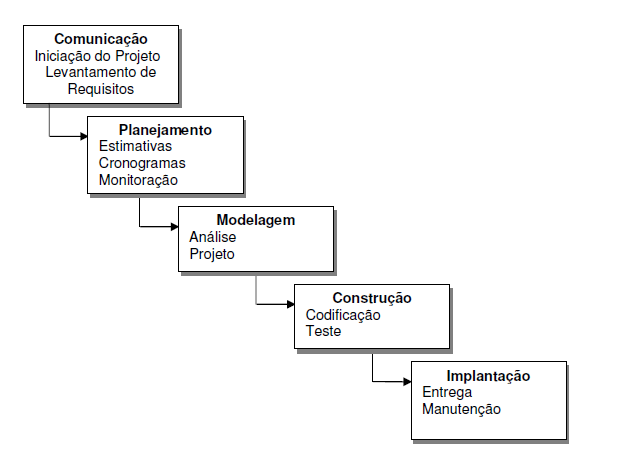
\includegraphics[width=10cm]{figuras/figura_ciclo_cascata}
\label{figura_ciclo_cascata}
\fnote{Fonte: \citeonline{pressman2006engenharia}}
\end{figure}

Dividimos o processo em nove atividades. A seguir, descreveremos brevemente cada uma delas:
\begin{enumerate}
	\item Iniciar Projeto: nessa atividade identificamos os objetivos do projeto, suas restri\c{c}\~oes, envolvidos, a organiza\c{c}\~ao da equipe de desenvolvimento e por \'ultimo realizamos uma 
reuni\~ao de in\'icio do projeto.
	\item Requisitos: nessa atividade realizamos o levantamento e an\'alise dos requisitos, sua documenta\c{c}\~ao, verifica\c{c}\~ao e valida\c{c}\~ao, al\'em de um estudo para saber atrav\'es dos 
requisitos se o projeto \'e vi\'avel. 
	\item Projeto: nessa atividade desenvolvemos o projeto da arquitetura do sistema, o planejamento dos m\'odulos, o projeto da interface gr\'afica com o usu\'ario  e como ser\~ao persistidos as 
entidades do sistema.
	\item Implementação: nessa atividade escolhemos primeiramente um m\'odulo do sistema para implementar, em seguida planejamos como ocorrer\'a a implementa\c{c}\~ao desse 
m\'odulo, implementamos o m\'odulo, e por \'ultimo realizamos a integra\c{c}\~ao de m\'odulo ao resto do sistema. Esse ciclo \'e repetido at\'e que todos os m\'odulos estejam desenvolvidos.
	\item Testes: durante essa atividade realizaremos o planejamento dos testes para o sistema, em seguida executaremos os testes para cada m\'odulo do sistema e para o sistema como um todo, e 
por \'ultimo iremos gerar um relat\'orio com os resultados dos testes.
	\item Implantação: ap\'os o sistema desenvolvido e devidamente testado, ele segue para a implanta\c{c}\~ao, em que prepararemos o ambiente onde o sistema ser\'a executado e realizaremos a 
implanta\c{c}\~ao. Ap\'os a implanta\c{c}\~ao, realizaremos testes de aceita\c{c}\~ao e a cria\c{c}\~ao de um manual para o sistema.
	\item Gerenciamento do Projeto: essa atividade ocorre durante todo o desenvolvimento do sistema e tem por objetivo permitir que o projeto consiga ser conclu\'ido dentro do prazo e da qualidade 
desejada.
	\item Avalia\c{c}\~ao do Processo: essa atividade \'e executada durante todo o desenvolvimento do projeto e permite que o processo utilizado seja constantemente avaliado e adaptado conforme segue 
o desenvolvimento do projeto.
	\item Encerrar Projeto: nessa \'ultima atividade ser\'a realizado apenas uma reuni\~ao em que ser\'a oficializado o final do projeto.
\end{enumerate}

O processo desenvolvido est\'a dispon\'ivel em \url{www.askmath.quixada.ufc.br/static/process/}. 

\subsection{Levantamento e Análise de Requisitos}


O Levantamento e An\'alise de Requisitos é a fase do desenvolvimento de um software em que o analista verifica junto ao usuário, quais as necessidades, condições e princípios que o \textit{software} 
deverá atender \cite{matuda2013mapas}. Essa fase possibilitou conhecer e estudar as necessidades do cliente, assim como as restrições que o software estará sujeito.

Para realizar a coleta dos requisitos, optamos por utilizar entrevistas com o cliente. Nessas entrevistas, que se caracterizarão como semi-estruturadas, já que foram guiadas por um roteiro previamente 
elaborado, composto por questões abertas \cite{belei2008uso}, foi possível obter os requisitos do sistema, assim como o público-alvo a quem o sistema atenderá. Essa técnica foi utilizada porque 
permitia uma organização flexível e ampliação dos questionamentos à medida que as informações foram sendo fornecidas pelo cliente \cite{fujisawa2000utilizaccao}.

O ambiente atender\'a quatro tipos de usu\'arios que formaram seu p\'ublico-alvo, ser\~ao administradores, professores, assistentes, e estudantes. Os administradores ser\~ao respons\'aveis por 
cadastrar 
novos professores, assim como realizar a manuten\c{c}\~ao di\'aria do sistema. Os professores ser\~ao responsáveis por definir as disciplinas e li\c{c}\~oes que faram parte do sistema. 
Ap\'os as disciplinas e li\c{c}\~oes definidas pelos professores, os assistentes ser\~ao respons\'aveis por manter os problemas de cada li\c{c}\~ao. Os estudantes resolver\~ao os problemas 
desenvolvidos pelos assistentes e poder\~ao postar d\'uvidas sobre qualquer conte\'udo no f\'orum de discuss\~oes. Quando o ambiente for aplicado em sala de aula, os professores ser\~ao ainda 
respons\'aveis por gerenciar suas turmas e acompanhar o andamento do progresso de cada um de seus estudantes, j\'a os assistentes ser\~ao responsáveis por tirar d\'uvidas dos estudantes no f\'orum 
de discuss\~oes.

Para uma melhor compreensão do público-alvo, foram criadas Personas 
\cite{pruitt2003personas}, personagens fictícios usados para caracterizar os papéis dos diferentes usuários do sistema \cite{guerra2010colaboraccao}. Cada persona criada possui um nome, hábitos, 
histórias pessoais, motivações, objetivos, entre outras (ver \nameref{apendice_personas}). A escolha dessa técnica deu-se pelo fato de que ela permitia ao desenvolvedor saber mais precisamente para 
quem ele deveria construir o sistema, além de permitir uma distinção maior do público-alvo e, dessa forma, aprofundar-se nos interesses individuais de cada um.

Apresentaremos a seguir, os principais requisitos levantados durante essa etapa:

\begin{alineascomponto}
	\item Hierarquia dos Conteúdos: no sistema, dever\~ao existir disciplinas, cada disciplina dever\'a possuir li\c{c}\~oes e cada li\c{c}\~ao ser\'a formada por problemas. Os professores poder\~ao 
cadastrar v\'arias disciplinas e li\c{c}\~oes, j\'a os assistentes ficar\~ao responsáveis por adicionar os problemas nas li\c{c}\~oes. Quando o estudante entrar no sistema, ele poder\'a ver somente 
as li\c{c}\~oes de uma disciplina por vez, podendo alternar entre disciplinas. Para um estudante come\c{c}ar a responder os problemas, ele dever\'a escolher inicialmente a disciplina e em seguida a 
li\c{c}\~ao. 

	\item Estrutura do Problema: cada problema possuir\'a uma descri\c{c}\~ao e v\'arios itens. Os problemas ser\~ao somente de m\'ultipla escolha e poder\~ao possuir no m\'inimo dois e no m\'aximo 
cinco itens, essa quantidade ficar\'a a crit\'erio do assistente que realizar\'a a adi\c{c}\~ao do problema no sistema.

	\item Saltar Problemas: o sistema deverá permitir ao aluno saltar problemas e rever os saltos 
realizados com algumas restrições na quantidade de saltos..
	
	\item Pedir Ajuda: para todo problema, o estudante poderá possuir uma ajuda. No momento em que o assistente estiver adicionando o problema, ele poderá ou não adicionar um texto de ajuda para o 
estudante, isso fica a critério dele. Quando o estudante estiver resolvendo os problemas, ele terá um botão que quando acionado, mostrar\'a o texto de ajuda. O sistema dever\'a salvar a quantidade 
de vezes que o estudante pedir ajuda e em quais problemas.
	
	\item Defici\^encias: \'e possível, a partir de um item respondido incorretamente em um problema, identificar a deficiência do estudante, por isso é fundamental que no momento que o 
assistente estiver adicionando os itens do problema, ele possa escolher para cada item incorreto, uma ou várias li\c{c}\~oes, essas lições ficarão sendo as supostas deficiências do aluno caso ele 
responda incorretamente aquele problema marcando aquele determinado item.
	
	\item F\'orum: o sistema deverá possuir um fórum onde os estudantes possam postar suas dúvidas para que professores, assistentes e outro participantes possam lhes ajudar com o problema. Esse fórum, deve possuir tópicos, comentários para os tópicos, e os comentários devem oferecer a opção de se comentar com imagens. 

\end{alineascomponto}

Após o levantamento dos requisitos, foi realizada a análise dos mesmos. Nessa análise, os requisitos foram agrupados em categorias. As categorias utilizadas são descritas por 
\citeonline{sommerville2003engenharia} como:
\begin{alineascomponto}
    \item Requisitos Funcionais -- especificam ações que um sistema deve ser
capaz de executar, sem levar em consideração restrições físicas. Os requisitos
funcionais especificam, portanto, o comportamento de entrada e saída de um
sistema.
    \item Requisitos Não Funcionais -- descrevem apenas atributos do sistema ou
atributos do ambiente do sistema, como segurança, desempenho, usabilidade e
confiabilidade.
    \item Requisitos de Domínio -- são os requisitos do domínio da aplicação do sistema e que refletem características desse domínio.
\end{alineascomponto}

Após esse agrupamento, os requisitos funcionais foram representados em Casos de Uso \cite{jacobson92engenharia}. Um caso de uso identifica os agentes envolvidos em uma interação e especifica o tipo 
de interação utilizando anotações sugeridas pela Unified Modeling Language (UML) 
\citeonline{sommerville2003engenharia}. Em seguida, foi realizada a documentação dos requisitos (ver \nameref{apendice_requisitos}).

No final dessa etapa, ocorreu a Validação dos Requisitos junto ao cliente.  A Validação dos Requisitos é definida como o processo que certifica que o modelo de requisitos gerado  esteja  consistente  
com  as  necessidades  e  intenções  de  clientes  e usuários \cite{rilston2003metodologia}. Esta etapa permitiu que os requisitos coletados e documentados estivesse de acordo com o que o 
cliente solicitou.

\subsection{Projeto do Sistema}

O Projeto de Software é à atividade de engenharia cujo foco é definir ``como'' os requisitos estabelecidos do projeto devem ser implementados no software \cite{pressman2006engenharia}. O objetivo da  atividade de projetar é gerar um modelo ou representação que apresente solidez, comodidade e deleite \cite{pressman2006engenharia}. 

Nesta fase, definimos como será aplicado o conhecimento obtido na pesquisa bibliográfica para se desenvolver o sistema. Para isto, definimos a arquitetura de software e as ferramentas que serão utilizadas durante o desenvolvimento do sistema. Nas seções a seguir, descrevemos um pouco sob cada um.

\subsubsection{Arquitetura}
Por arquitetura de software, entende-se a estrutura ou a organização de componentes de módulos, a maneira através da qual esses componentes interagem e a estrutura de dados que será usada pelos componentes \cite{pressman2006engenharia}.

A arquitetura utilizada baseia-se na arquitetura Cliente-Servidor\cite{david2013everything}, em que o processamento é dividido em processos distintos. Um processo é responsável pela manutenção da 
informação (servidor) e os outros são responsáveis pela captação de dados (clientes). Nessa arquitetura, os clientes enviam pedidos para o servidor, e este por sua vez processa estes dados e envia as 
respostas dos pedidos aos clientes.

Este modelo de arquitetura facilitará na manutenção do sistema, tendo em vista que toda atualização só necessitará ser realizada no servidor e automaticamente a mesma se propagará para todos os clientes. Com todos os recursos centralizados no servidor, podemos também ter um maior ganho com segurança, já que podemos centralizar os nossos esforços para manter a segurança das informações em apenas um único ponto, além de possibilitar que apenas cliente credenciados possam acessar e/ou alterar essas informações. Uma das outras grandes vantagens que temos  ao utilizar esse modelo, é que a medida que a quantidade de clientes aumente, será possível suprir esses clientes sem necessitar realizar nenhuma modificação essencial.

Para uma visualização mais detalhada da arquitetura de software definida, visitar o  \nameref{apendice_arquitetura}.

\subsubsection{Ferramentas}

 A análise do sistema foi feita com o auxílio da ferramenta de criação de diagramas Astah \cite{astah2016}, a implementação com a linguagem Python \cite{vanrossum2010python}, com o sistema de gerenciamento de banco de dados PostgresSQl \cite{momjian2001postgresql} e a camada de aplicação através da utilização do framework Django \cite{django2016}. Assim como a utilização do módulo Rosseta \cite{rosetta2016} para permitir a internacionalização do sistema.
 
A seguir, apresentaremos a lista das ferramentas e das tecnologias utilizadas para o desenvolvimento do projeto:

\begin{alineas}
	\item Astah: para a modelagem baseada em UML (Unified Modeling Language) do sistema.
	\item Python: linguagem de programação para implementação do sistema.
    \item Django: framework web responsável pela camada de aplicação.
    \item Rosetta: aplicação desenvolvida em Django que facilitará a tradução do projeto para diversas línguas.  
    \item PostgreSQL: como banco de dados para armazenamento e consulta de informações.
    \item Metro UI CSS: framework que faz uso de HTML, Cascading Stype Sheet (CSS) e Javascript para criação do front-end do sistema.
    \item MathJax: \'e uma engine\footnote{Uma biblioteca ou pacote de funcionalidades que são utilizadas para facilitar o desenvolvimento de alguma tecnologia.} de código aberto desenvolvido em 
javascript na forma de um plugin para incluir equações matemáticas em todos os navegadores, esse plugin aceita expressões em  MathML e Latex.

\end{alineas}

Essas ferramentas foram selecionadas por se tratarem, algumas, de ferramentas Open Source, ou seja, que seu código-fonte fonte pode ser alterado para diferentes fins, possibilitando assim que qualquer um consulte, examine ou as modifique, e outras por serem ferramentas que possibilitam um rápido desenvolvimento.

No final dessa etapa, foi gerado o Plano de Projeto, esse documento guiar\'a o desenvolvedor durante 
todo o processo de desenvolvimento.

\subsection{Implementação do Sistema}

A implementação envolve as atividades de codificação, compilação e integração. A codificação visa traduzir o design num programa, utilizando linguagens e  ferramentas adequadas. A codificação deve 
refletir a estrutura e o comportamento descrito no projeto. Os componentes arquiteturais devem ser codificados de forma independente e depois integrados \cite{aguiar2012requisitos}.

\subsection{Verificação e Validação}
Essa etapa destina-se a mostrar que o sistema está de acordo com a especificação 
e que ele atende às expectativas de clientes e usuários,  al\'em de assegurar 
que o  programa está fazendo aquilo que foi definido na sua especificação e que não 
possui  erros  de  execução \cite{aguiar2012requisitos}. 

Durante essa fase, ser\~ao realizados Testes de Unidade e Integra\c{c}\~ao em 
cada modulo do sistema, assim como Testes de Sistema no sistema j\'a integrado.

\citeonline{aniche2014teste} define essas categorias de Testes de Software como:

\begin{alineascomponto}
	\item Teste de Unidade -- é aquele que testa uma única unidade do sistema. 
Ele a testa de maneira isolada, geralmente simulando as prováveis dependências 
que aquela unidade tem. Em sistemas orientados a objetos, é comum que a unidade 
seja uma classe. Ou seja, quando queremos escrever testes de unidade para a 
classe Pedido, essa bateria de testes testará o funcionamento da classe Pedido, 
isolada, sem interações com outras classes.

	\item  Teste de Integração -- é aquele que testa a integração entre duas 
partes do seu sistema. Os testes que você escreve para a sua classe PedidoDao, 
por exemplo, em que seu teste vai até o banco de dados, é um teste de integração. 
Afinal, você está testando a integração do seu sistema com o sistema externo, 
que é o banco de dados. Testes que garantem que suas classes comunicam-se bem 
com serviços web, escrevem arquivos texto, ou mesmo mandam mensagens via socket 
são considerados testes de integração.

	\item Teste de Sistema -- \'e aquele que garante que o sistema funciona como um todo. Este 
nível de teste está interessado se o sistema funciona como um todo, com todas as 
unidades trabalhando juntas. Ele é comumente chamado de teste de caixa preta, já 
que durante o teste n\~ao se importa com a forma que os dados s\~ao processados, mas sim se as sa\'idas est\~ao de acordo com o que era esperado para entradas. 
\end{alineascomponto}

\subsection{Definição dos Conteúdo para o Sistema}

Após o sistema estar verificado e validado, ele terá que possuir conteúdos para ser utilizado pelo usuário final durante a fase de aplicação. A aplicação da primeira versão do sistema está planejada 
para ocorrer com uma turma de matemática da Universidade Federal do Ceará - Campus Quixadá. Decidimos optar por deixar os monitores\footnote{É o aluno de graduação concursado para exercer, juntamente 
com o professor, atividades técnico-didáticas condizentes com o seu grau de conhecimento junto à determinada disciplina, já por ele cursada.} da disciplina desenvolverem os conteúdos que ser\~ao 
utilizados no sistema durante essa fase. 

Os monitores passar\~ao por um treinamento, ao qual aprender\~ao a utilizar o sistema para, assim, adicionar os conteúdos desenvolvidos.

\subsection{Aplicação da Solução na Universidade Federal do Ceará - Campus Quixadá}

Aplicaremos o ambiente desenvolvido em duas turmas de Matemática Básica da UFC - Campus Quixadá. Nessas turmas, que est\'a previsto que sejam formadas por aproximadamente trinta estudantes 
cada, dividiremos os estudantes de cada turma em dois grupos, Grupo A1 e Grupo B1 para a primeira turma e Grupo A2 e B2 para a segunda turma. Os Grupos A1 e A2, ser\~ao formados pela metade 
dos estudantes de cada turma, escolhidos aleatoriamente, e os Grupos B1 e B2 pelos estudantes restantes. 
Esta divisão, deve-se ao fato de que ao final da experiência de utilização do ambiente pelos estudantes, realizaremos uma comparação no desempenho entre estudantes que utilizaram o sistema com os que 
não utilizaram. Dessa forma, o sistema será utilizado pelos estudantes dos Grupos A1 e A2, enquanto que os Grupos B1 e B2 (grupos de controle) continuaram estudando da mesma forma. 

O objetivo dessa experiência e analisar o impacto que o uso do ambiente desenvolvido tem na aprendizagem dos estudantes. Os dados que iremos utilizar para atingirmos os objetivos com essa 
experiência ser\~ao providos de duas avalia\c{c}\~oes realizadas por todos os alunos das duas turmas antes e depois a utiliza\c{c}\~ao do ambiente pelos Grupos A1 e A2.

\subsection{Cronograma de Execução}
\begin{table}[H]
\centering
\caption{Cronograma de Execução}
\label{cronograma}

\resizebox{\textwidth}{!}{
\begin{tabular}{|l|c|c|c|c|c|c|c|c|c|c|c|c|c|c|c|}
\hline
\multicolumn{1}{|c|}{\multirow{2}{*}{ATIVIDADES}} & \multicolumn{6}{c|}{2015} & \multicolumn{9}{c|}{2016} \\ \cline{2-16} 
\multicolumn{1}{|c|}{} & Jan & Fev & Mar & Abr & Mai & Jun - Dez & \multicolumn{1}{l|}{Jan - Mar} & \multicolumn{1}{l|}{Abr} & \multicolumn{1}{l|}{Mai} & \multicolumn{1}{l|}{Jun} & \multicolumn{1}{l|}{Jul} & \multicolumn{1}{l|}{Ago} & \multicolumn{1}{l|}{Set} & \multicolumn{1}{l|}{Out} & \multicolumn{1}{l|}{Nov} \\ \hline
Definição do Processo & x &  &  &  &  &  &  &  &  &  &  &  &  &  &  \\ \hline
Levantamento e Análise dos Requisitos & x & x & x &  &  &  &  &  &  &  &  &  &  &  &  \\ \hline
Projeto do Sistema &  &  &  & x & x &  &  &  &  &  &  &  &  &  &  \\ \hline
Implementação do Sistema &  &  &  &  &  & x & x & x & x & x &  &  &  &  &  \\ \hline
Verificação e Validação &  &  &  &  &  &  &  &  &  &  & x &  &  &  &  \\ \hline
Desenvolver o conteúdo para o sistema &  &  &  &  &  &  &  & x & x & x & x & x &  &  &  \\ \hline
Aplicação na UFC - Campus Quixadá &  &  &  &  &  &  &  &  &  &  &  & x & x & x &  \\ \hline
Definição do Projeto de Pesquisa &  &  &  &  &  &  &  & x &  &  &  &  &  &  &  \\ \hline
Defesa do Projeto de Pesquisa &  &  &  &  &  &  &  &  &  & x &  &  &  &  &  \\ \hline
Ajustes Solicitados &  &  &  &  &  &  &  &  &  &  & x &  &  &  &  \\ \hline
Análise dos Resultados Obtidos na Aplicação. &  &  &  &  &  &  &  &  &  &  &  &  &  &  & x \\ \hline
Defesa do Trabalho Final &  &  &  &  &  &  &  &  &  &  &  &  &  &  & x \\ \hline
\end{tabular}}
\fnote{Fonte: Elaborado pelo autor}
\end{table}

	\chapter{RESULTADOS}
\label{chap:resultados}

Nesta seção apresentaremos o resultado deste trabalho.

Definimos o processo que foi utilizado durante o desenvolvimento do sistema, coletamos, analisamos e validamos os requisitos do sistema e realizamos o projeto do sistema. 

Na implementação, desenvolvemos os módulos: 

\begin{alineascomponto}
    \item Gerenciador de Usuários: módulo responsável por gerenciar os usuários do sistema como professores, assistentes e alunos.
    \item Gerenciador de Turmas: módulo responsável por gerenciar as turmas de alunos do sistema.
    \item Gerenciador de Disciplinas: módulo responsável por gerenciar as disciplinas que serão cadastradas no sistema.
    \item Gerenciador de Lições: módulo responsável por gerenciar as lições que os professores irão cadastrar no sistema.
    \item Gerenciador de Questões: módulo responsável por gerenciar os problemas que os assistentes e professores poderão cadastrar para cada lição.
    \item Gerenciador de Pontuação: módulo responsável por gerenciar a pontuação ganha pelos alunos, assim como seu nível de experiência ao longo da utilização do sistema. 
    \item Fórum: módulo responsável por permitir que alunos postem dúvidas dos mais variados  assuntos relacionadas ao sistema, seja dúvidas em relação ao conteúdo apresentado em sala de aula, assim como informações sobre o sistema e sugestões.
    \item Gerenciador de Progresso: módulo responsável por acompanhar o andamento de cada estudante durante seu aprendizado e identificar os obstáculo epistemológicos enfrentados, indicando ao aluno 
a exist\^encia desses obst\'aculos e o(s) conte\'udo(s) que ele possui defici\^encia (causador(es) do obstáculo) para ele assim poder pausar o conte\'udo que est\'a estudando e voltar a 
estudar o(s) conte\'udo(s) que o sistema indicar.
	\item Gerador de Estatísticas: módulo responsável por gerar as estatísticas que o professor utilizará para acompanhar o andamento de suas turmas e alunos, assim como para o uso pelo estudante, 
que utilizará para acompanhar seu próprio progresso durante sua aprendizagem no sistema. 
\end{alineascomponto}

A seguir, apresentaremos algumas telas do sistema:

\begin{figure}[h!]
  \centering
  \begin{minipage}[b]{0.49\textwidth}
	\caption{Tela Inicial}
    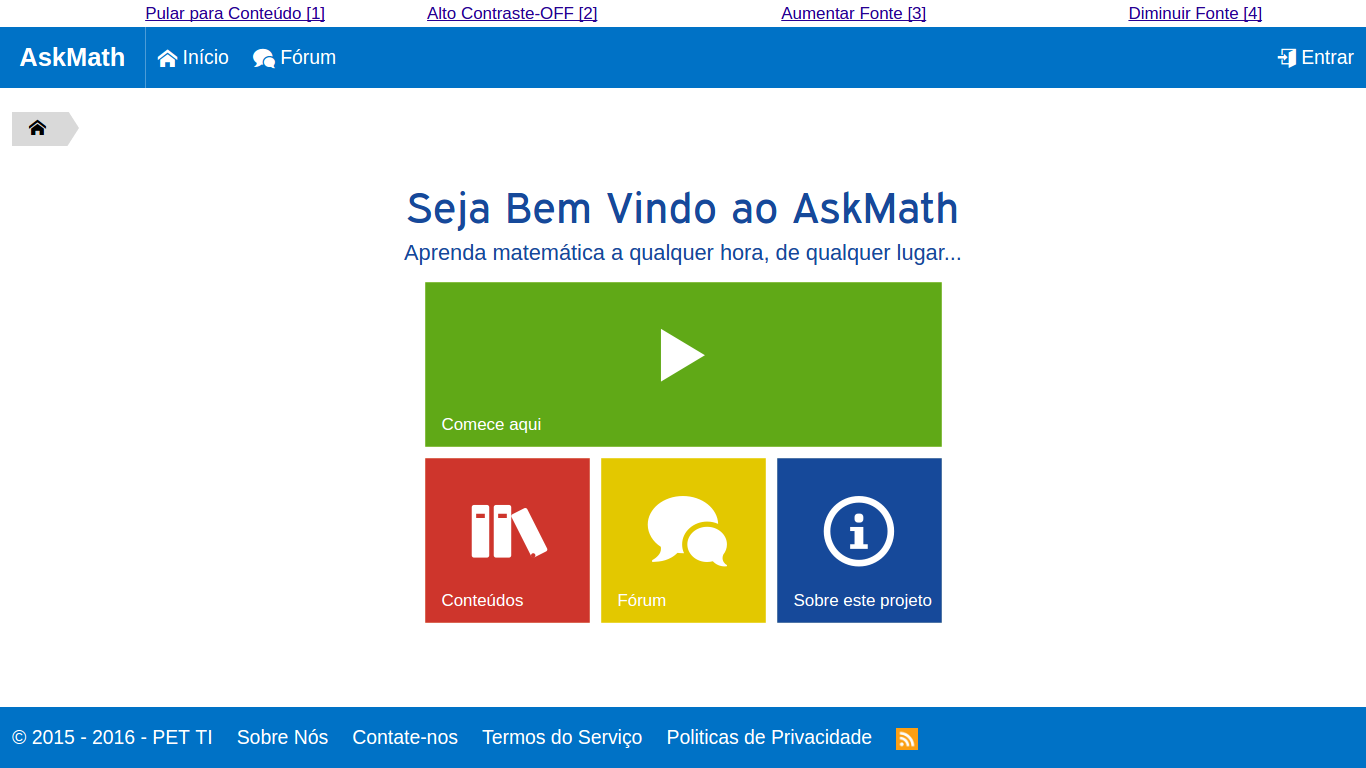
\includegraphics[width=\textwidth]{figuras/askmath/1}
  \end{minipage}
  \hfill
  \begin{minipage}[b]{0.49\textwidth}
	\caption{Tela Inicial do Estudante}
    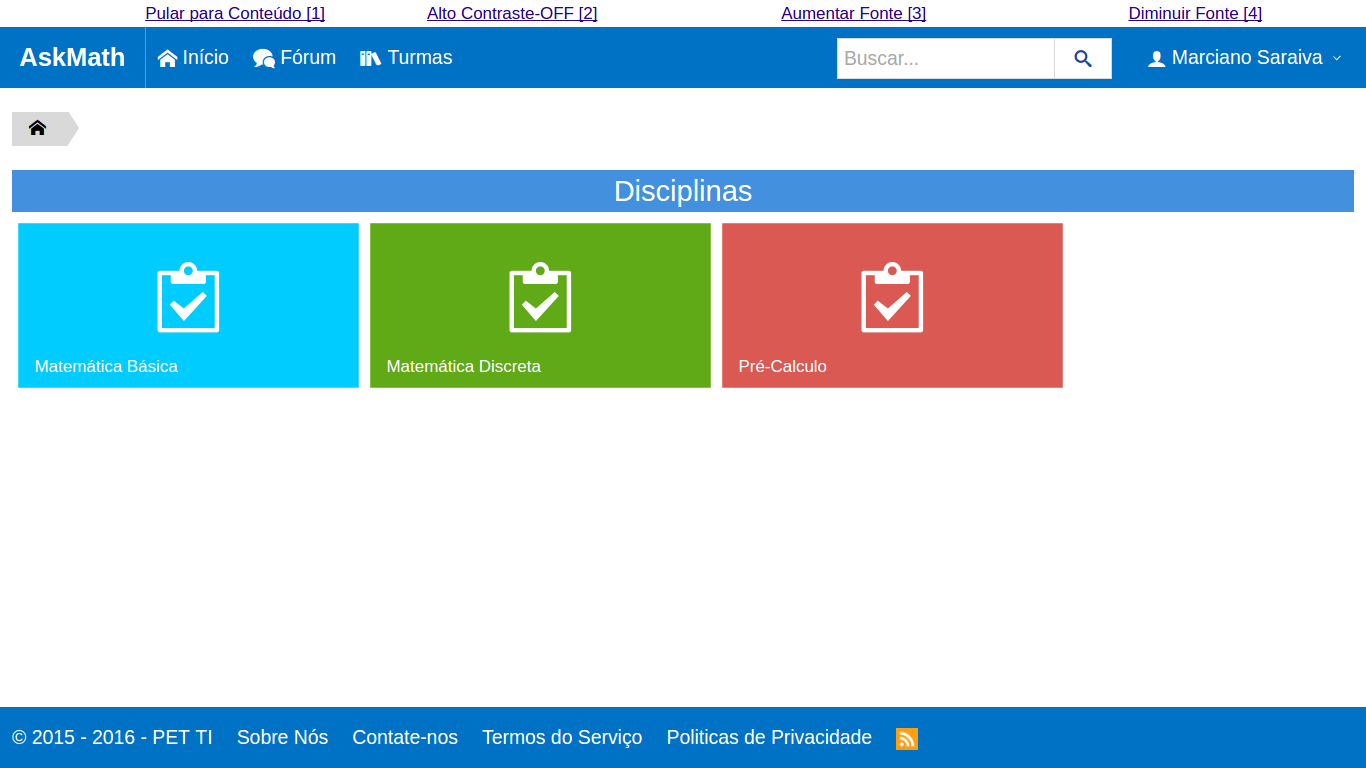
\includegraphics[width=\textwidth]{figuras/askmath/2}
  \end{minipage}
 
  \begin{minipage}[b]{0.49\textwidth}
    \caption{Tela de Administra\c{c}\~ao}
    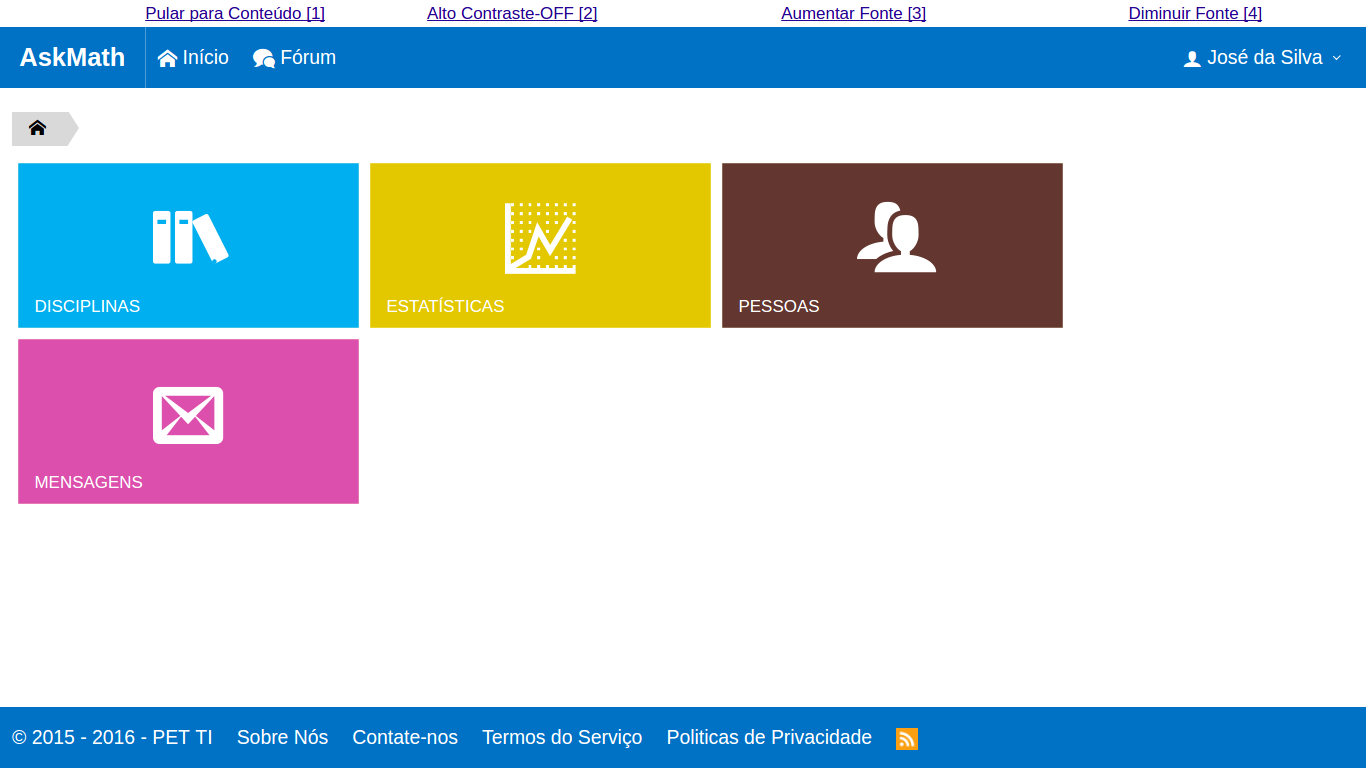
\includegraphics[width=\textwidth]{figuras/askmath/3}
  \end{minipage}
  \hfill
  \begin{minipage}[b]{0.49\textwidth}
	\caption{Tela de Problemas do Estudante}
    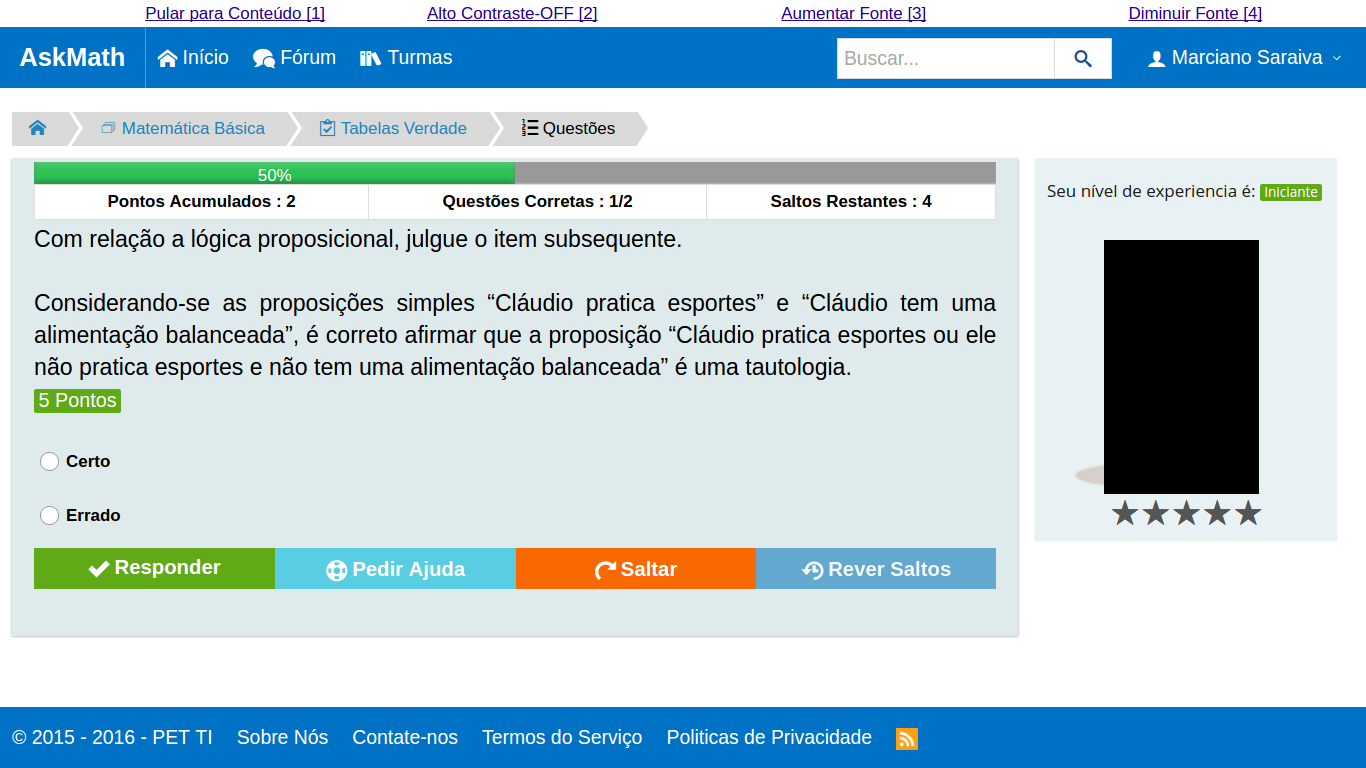
\includegraphics[width=\textwidth]{figuras/askmath/4}
  \end{minipage}
\end{figure}

[FALAR DA AVALIAÇÂO AQUI]
	\chapter{CONCLUSÕES E TRABALHOS FUTUROS}
\label{chap:conclusoes-e-trabalhos-futuros}

Esse capítulo apresenta as considerações finais a cerca desse trabalho. Além disso, é proposta a inclusão de novas funcionalidades que podem ser desenvolvidas em trabalhos futuros.

\section{Conclusões}

Após a implementação da solução proposta por este trabalho, constatou-se que tanto o objetivo geral quanto os específicos foram atendidos. O sistema foi desenvolvido conforme as melhores práticas e padrões em desenvolvimento de \textit{software} disponíveis no momento, tornando o sistema flexível, modularizado e reusável. Além disso, o sistema proporciona de fato um ambiente em que alunos podem práticar os conhecimentos adquiridos e até assimilar novos conhecimento. 

Finalmente, o sistema pode ainda ser utilizado como complemento ao ensino presencial, auxiliando professores e tutores no acompanhamento do aprendizado de seus alunos e apredizes.

Podem-se evidenciar limitações na solução desenvolvida na questão da comunicação entre aluno-aluno e aluno-profesor, já que isso só ocorre através do fórum de discurções, vale ressaltar que é improvável que, durante a aplicação do sistema, tais limitações sejam atingidas a ponto de comprometer a finalidade do sistema.

\section{Sugestões para Trabalhos Futuros}

No que tange trabalhos futuros que podem ser realizados baseando-se neste projeto, podem ser citados: desenvolver um módulo de bate-papo entre os alunos e professores, adição de conteúdos apresentados através de recursos visuais como vídeo, melhorias na \textit{interface} gráfica para aumentar a usabilidade do sistema. 

Por fim, pode-se avaliar o aprendizado que o sistema pode proporcionar à alunos durante seu uso como complemento ao ensino.




	
	%Elementos pós-textuais	
	\bibliography{elementos-pos-textuais/referencias}
%	\imprimirglossario	
	\imprimirapendices
		% Adicione aqui os apendices do seu trabalho
		\apendice{ TÍTULO}
\label{ap:TITULO}

Texto texto texto texto texto texto texto texto texto texto texto texto texto texto texto texto texto texto texto texto texto texto texto texto texto texto texto texto texto texto texto texto texto texto texto texto texto texto texto texto.
		\apendice{Modelo de Capa}
\label{ap:apendice_b}

Texto texto texto texto texto texto texto texto texto texto texto texto texto texto texto texto texto texto texto texto texto texto texto texto texto texto texto texto texto texto texto texto texto texto texto texto texto texto texto texto.

	\imprimiranexos
		% Adicione aqui os anexos do seu trabalho
		\anexo{Exemplo de Anexo}
\label{an:exemplo-de-anexo}

Texto texto texto texto texto texto texto  texto texto texto  texto texto texto  texto texto texto  texto texto texto  texto texto texto  texto texto texto  texto texto texto  texto texto texto  texto texto texto  texto texto texto. 		
		\anexo{Titulo anexo}
\label{an:anexo_b}

Texto texto texto texto texto texto texto texto texto texto texto.

	\imprimirindice

\end{document}